To test our algorithm, we use a standard benchmark set of multidimensional integrands proposed by Genz\footnote{\url{http://www.sfu.ca/~ssurjano}} \cite{Genz}, consisting of six families of functions with a set of parameters which can be varied to vary the level of difficulty of the integration problem. 

We examine the rate of convergence of our BART approach to BQ  when estimating the integrals in Eq.~\eqref{eq:integral} for each Genz family and compare it two baselines: Monte Carlo integration and Bayesian Quadrature with Gaussian processes. The Genz functions are defined on the unit $d$-dimensional hypercube $[0, 1]^d$ and this is taken as the domain of integration. For simplicity, we choose as our prior distribution $p(x)$ the uniform distribution over $[0, 1]^d$. The Genz functions have two sets of parameters, $d$ ``ineffective'' parameters $u$ and $d$ ``effective'' parameters $a$ which vary the level of difficulty. We use the default setting of $u = [0.5, \ldots, 0.5]^{\top}$ and re-scale $a$ suitably as the dimension increases to ensure numerical stability. Specifically, this is done by bounding the $L_1$-norm of $a$ so that numerical stability is obtained \cite{rescallingGenz}. To generate draws from $p(x)$ we use Latin Hypercube sampling \cite{Press:2007:NRE:1403886}. As ground truth, we analytically compute the integrals for these Genz test functions, which we include with further explanation in the Appendix. 

\subsection{Implementation Details}
\subsubsection{BART-BQ}
We use the \textit{bart} function in the \texttt{dbarts} package \cite{R} when implementing the BART model. We mostly use default hyperparameter settings, following \cite{BART}. However, we found that for our experiments, 50 trees was sufficient (as opposed to a default of 200). We also scaled the prior variance of the node parameters by $k=5$ (as opposed to a default of $k=2$) to ensure that a larger range of values can be assigned to the response for the difficult integration problems.

The prior of the node parameters, or the coefficients of the indicator functions, is given a Gaussian prior distribution in the Bayesian setting. Through the rescaling operation and the prior assignment, larger probability is assigned to the range of the response variable, following the works of \cite{BART}. The prior of the residual variance $\sigma$  receives an inverse chi-squared distribution $\nu\lambda/\chi^2_\nu$ with $(\nu, \lambda) = (3, 0.9)$ as suggested in \cite{BART}, which helps us avoid overfitting. Lastly, the size of tree is controlled by the parameters $\alpha$ and $\beta$ mentioned by \cite{CART}. We use the default setting $(0.95, 2)$ throughout the experiments.

To ensure the convergence of our MCMC procedure, we use a burn-in period of 1000 iterations, followed by 1000 draws. We then thin by a factor of 20 to obtain a final set of 50 draws. Finally, as the response data is implicitly scaled by the \textit{bart} function onto interval $[-0.5, 0.5]$ to optimize performance \cite{BART}, we re-scale them by the following inverse transformation 

\begin{equation}
    \hat{y}^{\ast} = (y^{\ast} + 0.5) (\boldsymbol{y}_{max} - \boldsymbol{y}_{min}) + \boldsymbol{y}_{min} .
\end{equation}

Starting from an initial sample of size 100, we implement sequential Bayesian Quadrature with Gaussian Process 500 times by iteratively selecting a new point using Algorithm~\ref{alg:SQ}.

\subsubsection{Sequential Bayesian Quadrature with Gaussian processes}
Our main competitor is Sequential Bayesian Quadrature with Gaussian processes (GP-BQ), the leading BQ approach presented in literature. It works by placing a Gaussian process prior on the integrand in Eq.~\eqref{eq:integral} (thus also on the integral $I_f$) and inference on the true integral value is made by considering the posterior mean and variance \cite{Rasmussen:2005:GPM:1162254}. As in BART-BQ, we refine this method through an active learning procedure. 500 new sample points that maximise the posterior sample variance are added sequentially via almost the same scheme. Furthermore, we choose the Gaussian kernel given by
\begin{align}
    k(x, x') = \sigma^2\text{exp}\left(-\frac{(x-x')^2}{2l^2}\right).
\end{align}
Ideally, hyperparameters should be learned, either by maximizing the marginal likelihood (the usual practice) or placing a prior on them and then sampling. However, for computational convenience, we set $\sigma = 1$ in all cases by standardizing the responses $y$ and apply the median heuristic, choosing the bandwidth $l$ as the median distance between points drawn from a uniform prior over the unit hypercube of dimension $d$.
Unfortunately, this default approach meant that we sometimes obtained negative posterior variances, a problem that has been discussed previously in the literature \cite{Rasmussen:2002:BMC:2968618.2968681}. Details of our complete formulation can be found in the appendix.

With an active procedure, although costly, it significantly increases the posterior concentration rate of the mean to the true integral value, as illustrated in Figure~\ref{fig:gpSeqDesign}. 

\begin{figure}[!bt]
    \centering
    \vspace*{-8mm}
    \includegraphics[width = 0.35\textwidth, angle = -90]{../../report/Figures/convergenceMean510DimensionsNoSeqDes.eps}
    \vspace*{-5mm}
    \caption{Convergence of the GP estimates of the oscillatory Genz family of dimension 10 with 12, 30, 50, 70 and 100 candidates for sequential design. The black dotted line is the true integral value.}
    \label{fig:gpSeqDesign}
    \vspace*{-1mm}
\end{figure}

\subsubsection{Monte Carlo Integration}
We further compare our method with the crude Monte Carlo estimation \cite{Press:2007:NRE:1403886}
\begin{equation}
    I_f \approx \frac{1}{n}\sum_{i = 1}^{n} f(x_i),
\end{equation}
where $x_i$ are again generated by Latin Hypercube sampling with sample size $n$ increasing from 1 to 500.

\subsection{Experimental Results}

% \begin{filecontents*}{bestMethods.csv}
% "","1","2","3","5","10","20"
% "cont","BARTBQ","MI","GPBQ","BARTBQ","MI","BARTBQ"
% "copeak","MI","MI","GPBQ","GPBQ","GPBQ","BARTBQ"
% "disc",NA,"BARTBQ","MI","BARTBQ","BARTBQ","BARTBQ"
% "gaussian","GPBQ","MI","BARTBQ","BARTBQ","GPBQ","MI"
% "oscil","MI","GPBQ","GPBQ","GPBQ","GPBQ","GPBQ"
% "prpeak","BARTBQ",NA,"GPBQ","BARTBQ","GPBQ","MI"
% \end{filecontents*}

%\tiny
%\begin{tabular}{l|l|l|l|l|l|l}
%     \bfseries Time (s) & \bfseries Zeroed %time% specify table head
%     \csvreader[head to column %names]{report/Writing/5.Model_Perform%ance/bestMethods.csv}{}% use head of %csv as column names
%     %\csvreader[head to column %names]{/}{}% use head of csv as %column names
%     {\\\hline\csvcoli&\csvcolii&\csvcolii%i&\csvcoliv&\csvcolv&\csvcolvi&\csvco%lvii}% specify your coloumns here
%\end{tabular}

%\begin{center}   
%\caption{Methods that give the best estimation in terms of the $L_1$ distance to the %true value on the last iteration. A full table estimates.}
%\vspace{2mm}
%    \scalebox{0.85} {
%    \begingroup\catcode`"=9
%    \csvautotabular{report/Writing/5.Model_Performance/bestMethods.csv}
%    \endgroup
%    }
%    \label{table:genz}
%\end{center}

\import{report/Writing/5.Model_Performance/}{rmseValues.tex}

Table~\ref{table:genz} shows the outcome of our benchmark tests for all six Genz families with dimensions $1$, $2$, $3$, $5$, $10$ and $20$. For illustration purposes, we only show a couple of the convergence plots and we refer the reader to the supplementary material for the full set of results. 

\begin{figure}[!t]
    \centering
    \vspace*{-12mm}
    \includegraphics[width = 0.36\textwidth, angle = -90]{../../report/Figures/3/convergenceMean320Dimensions.eps}
    \vspace*{-10mm}
    \caption{Convergence of the integral of the discontinuous Genz function of dimension 20 run with 500 epochs of sequential design. The true integral value is 0.2816, as indicated above.}
    \label{fig:genz2}
    \vspace*{-1mm}
\end{figure}

As would be expected theoretically, BART-BQ outperforms the other two methods when the function is non-smooth, e.g. the discontinuous family. Indeed, existing Bayesian quadrature methods are known to struggle when estimating discontinuous functions due to the need to tune hyperparameters and the choice of the kernel function (for GP-BQ) \cite{Rasmussen:2002:BMC:2968618.2968681}. Furthermore, both GP-BQ and Monte Carlo work well mostly for low dimensions ($<20$). There is a clear degradation in convergence for dimension 20 for our experiments, as shown in Table~\ref{table:genz}.
 
Figure~\ref{fig:genz2} displays the rate of convergence for the discontinuous family with dimension 20. Note that the posterior variance for GP empirically always tends to zero, as the predictive variance does not depend on the response \cite{Rasmussen:2005:GPM:1162254}, or even negative due to numerical issues \cite{Rasmussen:2002:BMC:2968618.2968681} and is out of scale, thus being omitted in the plot. %{(\color{red} The posterior variance of BART also stablises after 150 new data points, which results from the fact that we only take 100 posterior sample draws when running BART. (NEED TEST) )}
The BART-BQ estimates converge remarkably fast compared to GP-BQ. It also appears to be unbiased as opposed to a systematic bias exhibited by the GP estimator, which is most likely due to the undesired functional form of this family. The standard error of Monte Carlo estimates, on the other hand, decreases at the rate of $\frac{1}{\sqrt{N}}$, which is illustrated in Figure~\ref{fig:genz2}. But the standard error exhibited by crude Monte Carlo is still larger than BART-BQ. Note also that there is an abrupt decrease in the variance of BART-BQ. This may be due to the addition of a particular point in a previously unexplored region. 

\begin{figure}[!t]
    \centering
    \vspace*{0mm}
    \includegraphics[width = 0.3\textwidth, angle = -90]{../../report/Figures/runTimePlot.eps}
    \vspace*{-2mm}
    \caption{Run time of BART-BQ and GP-BQ with 500 additional samples collected using sequential design.}
    \label{fig:timePlot}
    \vspace*{-0.8em}
\end{figure}


BART-BQ is outperformed by GP-BQ when estimating the integral of the oscillatory family. We show the convergence plot for dimension 5 in Figure~\ref{fig:genz3} as an example. This result is probably due to the fact that the oscillatory family is relatively smooth, and so it can be modeled well by a Gaussian process with a smooth kernel  \cite{10.2307/25464673}, while BART is more appropriate for non-smooth functions. Nevertheless, the difference in performance between the two methods is significant.

% Investigating the convergence plots ({\color{InsertPlots}}), 
\begin{figure}[!ht]
\centering
\vspace*{-8mm}
\includegraphics[width = 0.35\textwidth, angle = -90]{../../report/Figures/5/convergenceMean55Dimensions.eps}
\vspace*{-5mm}
\caption{Convergence of the integral of the oscillatory Genz function of dimension 5 run with 500 epochs of sequential design. The actual integral is -0.08921 as indicated above.}
\label{fig:genz3}
\vspace*{-1mm}
\end{figure}

\subsection{Running time}
We compare the run time of BART-BQ to that of GP-BQ as we vary the dimensionality $d$ of the input space. As BART relies on an MCMC routine, which does not have a deterministic running time, we follow \cite{BART} and analyse its running time empirically in Figure~\ref{fig:timePlot}, where we average the run-times for all Genz families for a given dimension. We see that the time complexity of GP-BQ grows more rapidly as the dimension increases. than of that BART-BQ. This agrees with the empirical results in \cite{BART} which found that BART was relatively insensitive to the dimensionality.

GP-BQ is usually proposed in settings where it is costly to obtain samples, so the sample size is low and the $O(n^3)$ running time of GPs is not an issue. There are, however, certain settings in which $n$ might be very large---for example, a large set of initial samples, on the order of $10,000$ could be obtained through parallel random sampling. But for $n > 10,000$, GPs become too costly (without further approximations which may decrease the effectiveness of BQ). By contrast, BART was shown empirically to have $O(n)$ time complexity \cite{BART}. 

%The computational complexity of the GP is due to the fact that as we sample more candidates and increase dimensions of input for the sequential design, it becomes more difficult to invert the kernel matrix and perform the necessary calculations of to calculate the cumulative density using the R library \texttt{mvtnorm}, an already efficient package written in C and Fortran. It is also often the case that the kernel matrix becomes numerically singular, which is often resolved by adding a noise to the kernel matrix. However, to what extent this would affect our approximation of the integral as we obtain more samples is unknown. Indeed, since the run time of GP is mainly affected by \texttt{mvtnorm} packages while the run time of BART is only affected by the level of \textbf{for} loops (O($n^3$)), we expect a sharp decrease in BART's run time after rewriting the codes with RCpp.

%In practice, $p(x)$ may not be known and we are only able to sample from this distribution e.g.~ posterior distributions of the Gaussian process classification (logit) model or hierarchical generalised extreme value modelling. This is a major disadvantage of GP-BQ as we may not be able to use this method at all if it were this case. Whereas this problem is solve-able using Monte Carlo integration, we see that from Figures~\ref{fig:genz2} and \ref{fig:genz3} the standard deviation is a lot larger than that of BART-BQ.

% We are going to examine our model on how efficient it is in converging to the real value; how reliable the model is in terms of standard deviation and how well the model performs on high dimensional integral.